\chapter{Validation of the Approach}
Our proposed approach is validated by running it through three data sets based off of the data sets used by Hasda, R., Bhattacharjya, R., and Bennis, F. (2017) \cite{Hasda2017}, and Lee, Y., and Lee, M. \cite{Lee2002} that will test its performance and compare it to a genetic algorithm-based approach. Basing from previous studies, the fitness of the solution produced by an approach determines the performance of an algorithm. As such, we will be comparing the average fitness values of our approach and two competing approaches, a modified genetic algorithm approach, and a particle swarm optimization-based approach. 30 feasible solutions are obtained with each approach and data set, and the fitnesses obtained in each run are averaged. Note that, however, only the fitnesses of feasible solutions are included in the average. Due to the non-deterministic nature of metaheuristics, infeasible solutions are bound to be generated.

\section{Data Sets Used}
Let us call the data sets used as problem configuration. The first two problem configurations are based off of the configurations used by Hasda, R., Bhattacharjya, R., and Bennis, F. (2017) \cite{Hasda2017}. The first configuration used, which we will call SFLP-II, is shown in Table \ref{dataset-sflp-ii}, contains 8 buildings, and the second configuration, which we will call mSFLP-III, is shown in Table \ref{dataset-msflp-iii}, contains 20 buildings. The second configuration is called as such due to the fact that it is a modification of the third problem configuration used by Hasda, R., Bhattacharjya, R., and Bennis, F.. SFLP-II uses a 12x12 bounding region, while mSFLP-III uses a 260x260 bounding region. The third configuration, which we will call mLeeKra30a, is shown in Table \ref{dataset-mleekra30a}, contains 30 buildings. The configuration consists of modified building dimension data from the 30-building data set by Lee, Y., and Lee, M. \cite{Lee2002} and cost data from the Kra30a data set in QAPLIB \cite{QAPLib}. A 250x250 bounding region is used for the data set.

\begin{table}[h!]
\centering
\begin{tabular}{P{7mm}|P{7mm}|P{7mm}|P{7mm}|P{7mm}|P{7mm}|P{7mm}|P{7mm}|P{7mm}|P{7mm}|P{7mm}|}
	\cline{2-11}
	& \multicolumn{8}{c|}{Cost of Material Flow Between Buildings} & W & H \\ \cline{1-9}
	\multicolumn{1}{|l|}{Building} & 1     & 2     & 3     & 4     & 5     & 6     & 7     & 8    &       &        \\ \hline
	\multicolumn{1}{|l|}{1}        & 0     & 1     & 2     & 0     & 0     & 0     & 2     & 0    & 2     & 3      \\ \hline
	\multicolumn{1}{|l|}{2}        & 0     & 0     & 4     & 3     & 6     & 0     & 0     & 2    & 4     & 5      \\ \hline
	\multicolumn{1}{|l|}{3}        & 0     & 0     & 0     & 2     & 0     & 3     & 1     & 0    & 2     & 2      \\ \hline
	\multicolumn{1}{|l|}{4}        & 0     & 0     & 0     & 0     & 5     & 2     & 0     & 2    & 3     & 3      \\ \hline
	\multicolumn{1}{|l|}{5}        & 0     & 0     & 0     & 0     & 0     & 0     & 0     & 4    & 2     & 4      \\ \hline
	\multicolumn{1}{|l|}{6}        & 0     & 0     & 0     & 0     & 0     & 0     & 4     & 0    & 4     & 4      \\ \hline
	\multicolumn{1}{|l|}{7}        & 0     & 0     & 0     & 0     & 0     & 0     & 0     & 1    & 4     & 4      \\ \hline
	\multicolumn{1}{|l|}{8}        & 0     & 0     & 0     & 0     & 0     & 0     & 0     & 0    & 3     & 4      \\ \hline
\end{tabular}
\caption{Configuration of SFLP-II. W and H mean width and height, respectively.}
\label{dataset-sflp-ii}
\end{table}

\begin{table}
\begin{adjustwidth}{-0.85in}{}
\begin{tabular}{P{3mm}|P{3mm}|P{3mm}|P{3mm}|P{3mm}|P{3mm}|P{3mm}|P{3mm}|P{3mm}|P{3mm}|P{3mm}|P{3mm}|P{3mm}|P{3mm}|P{3mm}|P{3mm}|P{3mm}|P{3mm}|P{3mm}|P{3mm}|P{3mm}|P{3mm}|P{3mm}|}
	\cline{2-23}
	& \multicolumn{20}{c|}{Cost of Material Flow Between Buildings}                            & W & H \\ \cline{1-21}
	\multicolumn{1}{|l|}{Building} & 1 & 2 & 3 & 4 & 5 & 6 & 7 & 8 & 9 & 10 & 11 & 12 & 13 & 14 & 15 & 16 & 17 & 18 & 19 & 20 &       &        \\ \hline
	\multicolumn{1}{|l|}{1}        & 0 & 1 & 1 & 1 & 1 & 1 & 1 & 1 & 1 & 1  & 1  & 1  & 1  & 1  & 1  & 1  & 1  & 1  & 1  & 1  & 20    & 40     \\ \hline
	\multicolumn{1}{|l|}{2}        & 1 & 0 & 1 & 1 & 1 & 1 & 1 & 1 & 1 & 1  & 1  & 1  & 1  & 1  & 1  & 1  & 1  & 1  & 1  & 1  & 40    & 40     \\ \hline
	\multicolumn{1}{|l|}{3}        & 1 & 1 & 0 & 1 & 1 & 1 & 1 & 1 & 1 & 1  & 1  & 1  & 1  & 1  & 1  & 1  & 1  & 1  & 1  & 1  & 20    & 20     \\ \hline
	\multicolumn{1}{|l|}{4}        & 1 & 1 & 1 & 0 & 1 & 1 & 1 & 1 & 1 & 1  & 1  & 1  & 1  & 1  & 1  & 1  & 1  & 1  & 1  & 1  & 40    & 60     \\ \hline
	\multicolumn{1}{|l|}{5}        & 1 & 1 & 1 & 1 & 0 & 1 & 1 & 1 & 1 & 1  & 1  & 1  & 1  & 1  & 1  & 1  & 1  & 1  & 1  & 1  & 60    & 60     \\ \hline
	\multicolumn{1}{|l|}{6}        & 1 & 1 & 1 & 1 & 1 & 0 & 1 & 1 & 1 & 1  & 1  & 1  & 1  & 1  & 1  & 1  & 1  & 1  & 1  & 1  & 40    & 40     \\ \hline
	\multicolumn{1}{|l|}{7}        & 1 & 1 & 1 & 1 & 1 & 1 & 0 & 1 & 1 & 1  & 1  & 1  & 1  & 1  & 1  & 1  & 1  & 1  & 1  & 1  & 40    & 20     \\ \hline
	\multicolumn{1}{|l|}{8}        & 1 & 1 & 1 & 1 & 1 & 1 & 1 & 0 & 1 & 1  & 1  & 1  & 1  & 1  & 1  & 1  & 1  & 1  & 1  & 1  & 40    & 60     \\ \hline
	\multicolumn{1}{|l|}{9}        & 1 & 1 & 1 & 1 & 1 & 1 & 1 & 1 & 0 & 1  & 1  & 1  & 1  & 1  & 1  & 1  & 1  & 1  & 1  & 1  & 60    & 40     \\ \hline
	\multicolumn{1}{|l|}{10}       & 1 & 1 & 1 & 1 & 1 & 1 & 1 & 1 & 1 & 0  & 1  & 1  & 1  & 1  & 1  & 1  & 1  & 1  & 1  & 1  & 60    & 60     \\ \hline
	\multicolumn{1}{|l|}{11}       & 1 & 1 & 1 & 1 & 1 & 1 & 1 & 1 & 1 & 1  & 0  & 1  & 1  & 1  & 1  & 1  & 1  & 1  & 1  & 1  & 40    & 60     \\ \hline
	\multicolumn{1}{|l|}{12}       & 1 & 1 & 1 & 1 & 1 & 1 & 1 & 1 & 1 & 1  & 1  & 0  & 1  & 1  & 1  & 1  & 1  & 1  & 1  & 1  & 20    & 40     \\ \hline
	\multicolumn{1}{|l|}{13}       & 1 & 1 & 1 & 1 & 1 & 1 & 1 & 1 & 1 & 1  & 1  & 1  & 0  & 1  & 1  & 1  & 1  & 1  & 1  & 1  & 60    & 40     \\ \hline
	\multicolumn{1}{|l|}{14}       & 1 & 1 & 1 & 1 & 1 & 1 & 1 & 1 & 1 & 1  & 1  & 1  & 1  & 0  & 1  & 1  & 1  & 1  & 1  & 1  & 60    & 60     \\ \hline
	\multicolumn{1}{|l|}{15}       & 1 & 1 & 1 & 1 & 1 & 1 & 1 & 1 & 1 & 1  & 1  & 1  & 1  & 1  & 0  & 1  & 1  & 1  & 1  & 1  & 60    & 60     \\ \hline
	\multicolumn{1}{|l|}{16}       & 1 & 1 & 1 & 1 & 1 & 1 & 1 & 1 & 1 & 1  & 1  & 1  & 1  & 1  & 1  & 0  & 1  & 1  & 1  & 1  & 40    & 40     \\ \hline
	\multicolumn{1}{|l|}{17}       & 1 & 1 & 1 & 1 & 1 & 1 & 1 & 1 & 1 & 1  & 1  & 1  & 1  & 1  & 1  & 1  & 0  & 1  & 1  & 1  & 60    & 40     \\ \hline
	\multicolumn{1}{|l|}{18}       & 1 & 1 & 1 & 1 & 1 & 1 & 1 & 1 & 1 & 1  & 1  & 1  & 1  & 1  & 1  & 1  & 1  & 0  & 1  & 1  & 40    & 40     \\ \hline
	\multicolumn{1}{|l|}{19}       & 1 & 1 & 1 & 1 & 1 & 1 & 1 & 1 & 1 & 1  & 1  & 1  & 1  & 1  & 1  & 1  & 1  & 1  & 0  & 1  & 40    & 40     \\ \hline
	\multicolumn{1}{|l|}{20}       & 1 & 1 & 1 & 1 & 1 & 1 & 1 & 1 & 1 & 1  & 1  & 1  & 1  & 1  & 1  & 1  & 1  & 1  & 1  & 0  & 40    & 20     \\ \hline
\end{tabular}
\end{adjustwidth}
\caption{Configuration of mSFLP-III.}
\label{dataset-msflp-iii}
\end{table}

\begin{table}[h!]
\centering
\begin{adjustwidth}{0.3in}{}
\resizebox{0.85\textwidth}{!}{\rotatebox{90}{
\begin{tabular}{l|l|l|l|l|l|l|l|l|l|l|l|l|l|l|l|l|l|l|l|l|l|l|l|l|l|l|l|l|l|l|l|l|} 
	\cline{2-33}
	& \multicolumn{30}{c|}{Cost of Material Flow Between Buildings}         					  & W & H \\ \cline{1-31} \multicolumn{1}{|l|}{Building} & 1 & 2 & 3 & 4 & 5 & 6 & 7 & 8 & 9 & 10 & 11 & 12 & 13 & 14 & 15 & 16 & 17 & 18 & 19 & 20 & 21 & 22 & 23 & 24 & 25 & 26 & 27 & 28 & 29 & 30 &  &     \\ \hline
	\multicolumn{1}{|l|}{1}                                     & 0 & 2 & 2 & 2 & 2 & 2 & 2  & 2 & 3 & 0  & 3  & 2  & 0  & 0  & 0  & 3  & 3  & 0  & 0  & 2  & 1  & 2  & 1  & 1  & 0  & 3  & 0  & 0  & 0  & 0  & 56                 & 43                  \\ 
	\hline
	\multicolumn{1}{|l|}{2}                                     & 2 & 0 & 2 & 2 & 3 & 2 & 3  & 2 & 0 & 0  & 2  & 1  & 0  & 0  & 2  & 3  & 3  & 0  & 0  & 2  & 1  & 2  & 1  & 1  & 0  & 3  & 0  & 0  & 0  & 0  & 37                 & 43                  \\ 
	\hline
	\multicolumn{1}{|l|}{3}                                     & 2 & 2 & 0 & 2 & 2 & 3 & 0  & 0 & 0 & 0  & 2  & 2  & 0  & 0  & 2  & 3  & 3  & 0  & 0  & 2  & 1  & 2  & 1  & 1  & 0  & 3  & 0  & 0  & 0  & 0  & 78                 & 47                  \\ 
	\hline
	\multicolumn{1}{|l|}{4}                                     & 2 & 2 & 2 & 0 & 0 & 2 & 2  & 3 & 1 & 0  & 0  & 2  & 1  & 0  & 0  & 4  & 3  & 0  & 0  & 2  & 1  & 2  & 1  & 1  & 0  & 3  & 0  & 0  & 0  & 0  & 40                 & 20                  \\ 
	\hline
	\multicolumn{1}{|l|}{5}                                     & 2 & 3 & 2 & 2 & 0 & 2 & 3  & 2 & 0 & 0  & 2  & 1  & 0  & 0  & 2  & 3  & 3  & 0  & 0  & 2  & 1  & 2  & 1  & 1  & 0  & 3  & 0  & 0  & 0  & 0  & 42                 & 50                  \\ 
	\hline
	\multicolumn{1}{|l|}{6}                                     & 2 & 2 & 3 & 2 & 2 & 0 & 0  & 0 & 0 & 0  & 2  & 2  & 0  & 0  & 2  & 3  & 3  & 0  & 0  & 2  & 1  & 2  & 1  & 1  & 0  & 3  & 0  & 0  & 0  & 0  & 50                 & 35                  \\ 
	\hline
	\multicolumn{1}{|l|}{7}                                     & 2 & 3 & 0 & 3 & 3 & 0 & 0  & 4 & 4 & 3  & 3  & 0  & 4  & 0  & 0  & 2  & 2  & 0  & 0  & 3  & 4  & 1  & 0  & 0  & 0  & 0  & 0  & 0  & 0  & 0  & 20                 & 18                  \\ 
	\hline
	\multicolumn{1}{|l|}{8}                                     & 2 & 2 & 0 & 1 & 2 & 0 & 4  & 0 & 0 & 0  & 0  & 2  & 0  & 0  & 0  & 3  & 3  & 0  & 0  & 3  & 1  & 1  & 0  & 0  & 0  & 0  & 0  & 0  & 0  & 0  & 40                 & 39                  \\ 
	\hline
	\multicolumn{1}{|l|}{9}                                     & 3 & 0 & 0 & 0 & 0 & 0 & 4  & 0 & 0 & 0  & 0  & 1  & 4  & 0  & 0  & 2  & 2  & 0  & 0  & 2  & 0  & 1  & 0  & 0  & 0  & 0  & 0  & 0  & 0  & 0  & 40                 & 50                  \\ 
	\hline
	\multicolumn{1}{|l|}{10}                                    & 0 & 0 & 0 & 0 & 0 & 0 & 3  & 0 & 0 & 0  & 0  & 0  & 0  & 0  & 0  & 0  & 0  & 0  & 0  & 0  & 0  & 1  & 1  & 0  & 0  & 0  & 0  & 4  & 0  & 0  & 40                 & 49                  \\ 
	\hline
	\multicolumn{1}{|l|}{11}                                    & 3 & 2 & 2 & 2 & 2 & 2 & 3  & 0 & 0 & 0  & 0  & 3  & 4  & 0  & 0  & 3  & 3  & 0  & 0  & 0  & 1  & 2  & 0  & 0  & 0  & 2  & 0  & 0  & 0  & 0  & 40                 & 40                  \\ 
	\hline
	\multicolumn{1}{|l|}{12}                                    & 2 & 1 & 2 & 1 & 1 & 2 & 0  & 2 & 1 & 0  & 3  & 0  & 3  & 0  & 0  & 1  & 1  & 0  & 0  & 0  & 0  & 2  & 2  & 0  & 0  & 0  & 0  & 0  & 0  & 0  & 32                 & 28                  \\ 
	\hline
	\multicolumn{1}{|l|}{13}                                    & 0 & 0 & 0 & 0 & 0 & 0 & 4  & 0 & 4 & 0  & 4  & 3  & 0  & 4  & 0  & 3  & 3  & 0  & 0  & 2  & 1  & 1  & 1  & 0  & 0  & 0  & 0  & 4  & 0  & 0  & 30                 & 30                  \\ 
	\hline
	\multicolumn{1}{|l|}{14}                                    & 0 & 0 & 0 & 0 & 0 & 0 & 0  & 0 & 0 & 0  & 0  & 0  & 4  & 0  & 0  & 0  & 0  & 4  & 0  & 0  & 0  & 1  & 0  & 0  & 0  & 3  & 0  & 0  & 0  & 0  & 50                 & 50                  \\ 
	\hline
	\multicolumn{1}{|l|}{15}                                    & 0 & 2 & 2 & 4 & 2 & 2 & 0  & 0 & 0 & 0  & 0  & 0  & 0  & 0  & 0  & 1  & 1  & 0  & 0  & 0  & 0  & 2  & 0  & 0  & 0  & 3  & 0  & 2  & 0  & 0  & 20                 & 20                  \\ 
	\hline
	\multicolumn{1}{|l|}{16}                                    & 3 & 3 & 3 & 3 & 3 & 3 & 2  & 3 & 2 & 0  & 3  & 1  & 3  & 0  & 1  & 0  & 5  & 2  & 0  & 0  & 0  & 1  & 0  & 0  & 0  & 2  & 0  & 0  & 0  & 0  & 17                 & 18                  \\ 
	\hline
	\multicolumn{1}{|l|}{17}                                    & 3 & 3 & 3 & 3 & 3 & 3 & 2  & 3 & 2 & 0  & 3  & 1  & 3  & 0  & 1  & 4  & 0  & 2  & 0  & 0  & 0  & 1  & 0  & 0  & 0  & 2  & 0  & 0  & 0  & 0  & 20                 & 20                  \\ 
	\hline
	\multicolumn{1}{|l|}{18}                                    & 0 & 0 & 0 & 0 & 0 & 0 & 0  & 0 & 0 & 0  & 0  & 0  & 0  & 4  & 0  & 2  & 2  & 0  & 0  & 0  & 0  & 1  & 0  & 0  & 2  & 4  & 4  & 0  & 0  & 0  & 30                 & 30                  \\ 
	\hline
	\multicolumn{1}{|l|}{19}                                    & 0 & 0 & 0 & 0 & 0 & 0 & 0  & 0 & 0 & 0  & 0  & 0  & 0  & 0  & 0  & 0  & 0  & 0  & 0  & 0  & 0  & 0  & 0  & 0  & 0  & 0  & 0  & 0  & 2  & 0  & 25                 & 18                  \\ 
	\hline
	\multicolumn{1}{|l|}{20}                                    & 2 & 2 & 2 & 2 & 2 & 2 & 3  & 3 & 2 & 0  & 0  & 0  & 2  & 0  & 0  & 0  & 0  & 0  & 0  & 0  & 1  & 0  & 0  & 0  & 0  & 0  & 0  & 0  & 3  & 0  & 31                 & 16                  \\ 
	\hline
	\multicolumn{1}{|l|}{21}                                    & 1 & 1 & 1 & 1 & 1 & 1 & 4  & 1 & 0 & 0  & 1  & 0  & 1  & 0  & 0  & 0  & 0  & 0  & 0  & 1  & 0  & 1  & 2  & 0  & 0  & 0  & 0  & 0  & 4  & 0  & 43                 & 37                  \\ 
	\hline
	\multicolumn{1}{|l|}{22}                                    & 2 & 2 & 2 & 2 & 2 & 2 & 1  & 1 & 1 & 1  & 2  & 2  & 1  & 1  & 2  & 1  & 1  & 1  & 0  & 0  & 1  & 0  & 1  & 0  & 0  & 0  & 0  & 0  & 0  & 0  & 32                 & 28                  \\ 
	\hline
	\multicolumn{1}{|l|}{23}                                    & 1 & 1 & 1 & 1 & 1 & 1 & 0  & 0 & 0 & 1  & 0  & 2  & 1  & 0  & 0  & 0  & 0  & 0  & 0  & 0  & 2  & 1  & 0  & 0  & 0  & 0  & 0  & 0  & 4  & 0  & 30                 & 30                  \\ 
	\hline
	\multicolumn{1}{|l|}{24}                                    & 1 & 1 & 1 & 1 & 1 & 1 & 0  & 0 & 0 & 0  & 0  & 0  & 0  & 0  & 0  & 0  & 0  & 0  & 0  & 0  & 0  & 0  & 0  & 0  & 2  & 0  & 0  & 0  & 4  & 0  & 52                 & 48                  \\ 
	\hline
	\multicolumn{1}{|l|}{25}                                    & 0 & 0 & 0 & 0 & 0 & 0 & 0  & 0 & 0 & 0  & 0  & 0  & 0  & 0  & 0  & 0  & 0  & 2  & 0  & 0  & 0  & 0  & 0  & 2  & 0  & 4  & 0  & 0  & 0  & 0  & 20                 & 20                  \\ 
	\hline
	\multicolumn{1}{|l|}{26}                                    & 3 & 3 & 3 & 3 & 3 & 3 & 0  & 0 & 0 & 0  & 2  & 0  & 0  & 3  & 3  & 2  & 2  & 4  & 0  & 0  & 0  & 0  & 0  & 0  & 5  & 0  & 0  & 0  & 0  & 4  & 17                 & 18                  \\ 
	\hline
	\multicolumn{1}{|l|}{27}                                    & 0 & 0 & 0 & 0 & 0 & 0 & 0  & 0 & 0 & 0  & 0  & 0  & 0  & 0  & 0  & 0  & 0  & 4  & 0  & 0  & 0  & 0  & 0  & 0  & 0  & 0  & 0  & 0  & 0  & 0  & 20                 & 20                  \\ 
	\hline
	\multicolumn{1}{|l|}{28}                                    & 0 & 0 & 0 & 0 & 0 & 0 & 0  & 0 & 0 & 4  & 0  & 0  & 4  & 0  & 2  & 0  & 0  & 0  & 0  & 0  & 0  & 0  & 0  & 0  & 0  & 0  & 0  & 0  & 0  & 0  & 30                 & 30                  \\ 
	\hline
	\multicolumn{1}{|l|}{29}                                    & 0 & 0 & 0 & 0 & 0 & 0 & 0  & 0 & 0 & 0  & 0  & 0  & 0  & 0  & 0  & 0  & 0  & 0  & 2  & 3  & 4  & 0  & 4  & 4  & 0  & 0  & 0  & 0  & 0  & 0  & 22                 & 21                  \\ 
	\hline
	\multicolumn{1}{|l|}{30}                                    & 0 & 0 & 0 & 0 & 0 & 0 & 00 & 0 & 0 & 0  & 0  & 0  & 0  & 0  & 0  & 0  & 0  & 0  & 0  & 0  & 0  & 0  & 0  & 0  & 0  & 4  & 0  & 0  & 0  & 0  & 18                 & 28                  \\
	\hline
\end{tabular}}}
\end{adjustwidth}
\caption{Configuration of mKra30a. W and H mean width and height, respectively.}
\label{dataset-mleekra30a}
\end{table}

\section{Competing Approaches}
In order for us to properly gauge the performance of our GWO approach for the unequal area static facility layout problem, we will be solving the problem configurations using two other approaches: (1) a modified genetic algorithm approach, and a particle swarm optimization-based approach. These two were chosen due to their popularity in solving facility layout problems \cite{Hosseini-Nasab2018}.

\subsection{Modified Genetic Algorithm Approach}
The competing GA approach, which we will compare our proposed GWO approach, contains multiple phases to solve the unequal area static facility layout problem. The basic framework of the algorithm is inspired from the works of Asl et al. (2015) \cite{Asl2015} and Asl, A. and Wong, K. (2015) \cite{Asl2015a}. We will be further discussing the algorithm in detail in this section.

\subsubsection{Population Generation}
In the competing GA approach, the population generation is the same the method for initialization the population as the one in our proposed modified GWO approach.

\subsubsection{Swapping Method}
The swapping method is used to find a possible configuration for a solution that is better than the current configuration. This method is applied to all solutions in the population, but only in the first 100 iterations. Pseudocode for the swapping method is provided in Algorithm \ref{pseudocode-comp-ga-swapping}.

\begin{algorithm}
\caption{Pseudocode for the swapping method.}
\label{pseudocode-comp-ga-swapping}
\begin{algorithmic}[1]
\State Let $S$ be the collection of generated solutions.
\State Set $S_{curr}$ be the current solution.
\State Add $S_{curr}$ to $S$.
\State Set $N_{B}$ be the maximum number of buildings.
\For{i = 0 until $N_{B} - 2$}
	\For{j = i + 1 until $N_{B} - 1$}
		\State Building $i$'s orientation in $S_{curr}$ is changed to the other orientation,\WRP and the resulting new solution is added to $S$
		\State Building $j$'s orientation in $S_{curr}$ is changed to the other orientation,\WRP and the resulting new solution is added to $S$
		\State Building $i$'s and $j$'s orientations in $S_{curr}$ are changed to the other\WRP orientation, and the resulting new solution is added to $S$
		\State Building $i$'s and $j$'s positions are exchanged in $S_{curr}$, and the resulting new\WRP solutiA movement and a orientation changeon is added to $S$.
		\State Building $i$'s and $j$'s positions are exchanged in and the orientation of\WRP building $i$ is changed in $S_{curr}$, and the resulting new solution\WRP is added to $S$.
		\State Building $i$'s and $j$'s positions are exchanged in and the orientation of\WRP building $j$ is changed in $S_{curr}$, and the resulting new solution\WRP is added to $S$.
		\State Building $i$'s and $j$'s positions are exchanged in and the orientations of\WRP buildings $i$ and $j$ are changed in $S_{curr}$, and the resulting new solution\WRP is added to $S$.
	\EndFor
\EndFor \\
\Return the best solution in $S$.
\end{algorithmic}
\end{algorithm}

\subsubsection{Selection, Crossover, Mutation, and Elitism}
Key parts of a genetic algorithm are the selection, crossover, and mutation operators. These drive the algorithm to produce good solutions. We will be discussing each operator used in detail in this section. Elitism is also implemented in our proposed approach to ensure that the best solutions found so far do not get lost throughout iterations. It will also be discussed in this section.

\paragraph{Selection}
The selection operator used in the competing approach is tournament selection. Tournament selection works by selecting $k$ (also known as tournament size) individuals from a population and using the best two selected individuals as parents for an offspring \cite{StackOverflow-TournamentSelection}. Algorithm \ref{pseudocode-tournament-selection} shows a pseudocode of tournament selection. Note that in the algorithm, $P_{p}$ denotes the $p$-th solution in $P$, and $|P|$ denotes the population size.

\begin{algorithm}
\caption{Pseudocode for the tournament selection.}
\label{pseudocode-tournament-selection}
\begin{algorithmic}[1]
\State Set $X^{(1)}$ to be the first best parent.
\State Set $X^{(2)}$ to be the second best parent.
\State Set $P$ to be the population of solutions.
\State Set $k$ to be the tournament size.
\State Set $f(X)$ to be the fitness function.
\State $X^{(1)} = \text{null}$
\State $X^{(2)} = \text{null}$
\For{$i = 1, 2,\ldots,k$}
	\State $p = U(1, |P|)$
	\If{$X^{(1)}== \text{null}$ or $f(P_{p}) < f(X^{(1)}$}
		\State $X_{(2)} = X^{(1)}$
		\State $X_{(1)} = P_{p}$
	\ElsIf{$X^{(2)}== \text{null}$ or $f(P_{p}) < f(X^{(2)}$}
		\State $X_{(2)} = P_{p}$
	\EndIf
\EndFor \\
\Return $X^{(1)}$, and $X^{(2)}$.
\end{algorithmic}
\end{algorithm}

\paragraph{Crossover}
The crossover operator used in the competing approach is uniform crossover. Uniform crossover works by selecting a gene from a random parent and placing it in the offspring. This is applied for every gene in the offspring. Algorithm \ref{pseudocode-uniform-crossover} shows a pseudocode of uniform crossover.

\begin{algorithm}
\caption{Pseudocode for the uniform crossover.}
\label{pseudocode-uniform-crossover}
\begin{algorithmic}[1]
\State Set $X$ to be the offspring.
\State Set $N$ to be the number of genes a solution has.
\State Set $X^{(1)}$ to be the first parent.
\State Set $X^{(2)}$ to be the second parent.
\For{$i = 1, 2,\ldots, N$}
	\State $\text{rand} = U(0, 1)$
	\If{$\text{rand} < 0.5$}
		\State $X_{i} = X^{(1)}_{i}$
	\Else
		\State $X_{i} = X^{(2)}_{i}$
	\EndIf
\EndFor \\
\Return $X$.
\end{algorithmic}
\end{algorithm}

\paragraph{Mutation}
Over time, as more and more iterations are performed, the diversity of the population will eventually be lost. To combat this, a mutation operator is performed to reintroduce diversity. The mutation operator used is an operator that we dub the "Buddy-Buddy Mutation".

The \textbf{Buddy-Buddy Mutation} is a mutation operator that simply selects two pairs of buildings $D$ and $S$, and move one of them to the side of the other building. Building $D$ is referred to as the dynamic buddy, while building $S$ is referred to as the static buddy. Building $D$ will be the building that will be moved towards the other building, which is building $S$ in our case. When moving building $D$, a side $E$ of building $S$ will first be randomly chosen. Afterwards, an orientation for building $D$ will be randomly chosen, whether it will be parallel or perpendicular to $E$. Once a side and orientation has been selected, building $D$ will be moved adjacent towards building $S$ at side $E$ with the chosen orientation. The implementation of this mutation operator in our proposed approach gives buildings that intersect with another building more chances of being selected as the dynamic buddy. Pseudocode and a visualization of the operator is provided by Algorithm \ref{pseudocode-buddybuddy-mutation} and Figure \ref{buddy-buddy-mutation-viz}, respectively.

\begin{algorithm}
\caption{Pseudocode for the Buddy-Buddy Mutation.}
\label{pseudocode-buddybuddy-mutation}
\begin{algorithmic}[1]
	\State Randomly select two buildings $D$ and $S$, with more weight given to buildings that are intersecting with another.
	\State Set $E$ to be a randomly selected side of building $S$.
	\State Set $O$ to either be a parallel or perpendicular orientation, randomly selected.
	\State Move building $D$ adjacent to side $E$ of building $S$ with the orientation $O$.
\end{algorithmic}
\end{algorithm}

\begin{figure}[h!]
	\centering
	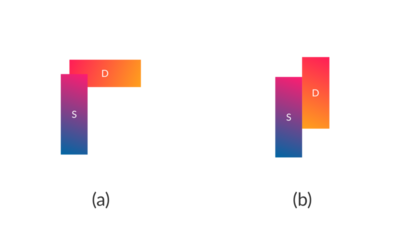
\includegraphics{./images/chap06-validation/buddy-buddy-mutation.png}
	\caption{Visualization of how Buddy-Buddy Mutation works. On the left are two buildings that are overlapping one another. The right shows the same buildings but with the mutation applied, causing them to no longer overlap. Note that the right shows only one possible arrangement for both buildings.}
	\label{buddy-buddy-mutation-viz}
\end{figure}

The rate at which a solution is mutated is highly dependent on the fitness of the solution. The worse the fitness of a solution is, the more likely it is to be mutated. This encourages the proposed algorithm to improve solutions that are generally bad. This rate scheme makes this an adaptive mutation operator \cite{Jiang2018}. The mutation rate is mathematically modelled as:

\begin{equation}
	m(X, t) = 1 - \frac{fit_{max}(t) - fit(X(t))}{fit_{max}(t) - fit_{min}(t)}
\end{equation}

where $m_{k}$ refers to the mutation rate of a solution $X$ at iteration $t$, $fit$ is a function that gets the fitness of a solution, and $fit_{min}$ and $fit_{max}$ gets the minimum and maximum fitnesses of the population, respectively.

\paragraph{Elitism}
One variant of genetic algorithms includes elitism. This elitism allows a genetic algorithm to keep a number of best solutions in the next generation, ensuring that the best solutions do not get discarded over time. Note that this elitism strategy is not only limited to genetic algorithms. Other evolutionary algorithms may also utilize this strategy \cite{Du2018}. We are also taking this principle into our competing GA approach. In the competing approach, we are keeping the best $E_{N}$ solutions in the previous iteration to the next iteration.

\subsubsection{Local Searches}
Remember that our implementation is based on aforementioned previous works that used local search algorithms in conjunction to genetic algorithms. They combined GAs with local search algorithms because GAs find it hard to explore within the convergence area. Hybridizing it with a local search algorithm improves performance \cite{Ripon2013}. In our proposed approach, we are keeping this aspect of the previous works. This will also ensure that we are able to search within the convergence area more intensely and find better solutions. In the previous works and in ours, there are two local search algorithms, dubbed "Local Search 1" and "Local Search 2". They vary in terms of searching intensity, but both attempts to obtain better solutions. We will be discussing details of both in this section.

\paragraph{Local Search 1}
The first local search algorithm, "Local Search 1", performs a local search by creating a number of solutions by moving each building in different directions by a certain random amount and changing its orientations after movement and obtaining the best solution from these activities. In our approach, the certain amount of movement is a random number between 1 and 5. This search algorithm is only applied to the best solution of the current iteration, and the best solution found in this search becomes the new best solution and replaces the previously best solution. The movements of each building is defined by a set of "activities". This set of activities is shown by Table \ref{local-search-1-activities}. Additionally, pseudocode of the search algorithm is shown in Algorithm \ref{pseudocode-local-search-1}.

\begin{table}[h!]
	\centering
	\begin{tabular}{| c | p{110mm} |}
		\hline
		Activity Number & Description \\
		\hline
		0 & A building is moved to the right along the x-axis by a random number between 1 and 5. \\
		1 & A building is moved to the left along the x-axis by a random number between 1 and 5. \\
		2 & A building is moved to the upwards along the y-axis by a random number between 1 and 5. \\
		3 & A building is moved to the downwards along the y-axis by a random number between 1 and 5. \\
		4 & Generate two random numbers from 1 and 5 and a building is moved to the right and then upward, respectively, by those numbers. \\
		5 & Generate two random numbers from 1 and 5 and a building is moved to the right and then downward, respectively, by those numbers. \\
		6 & Generate two random numbers from 1 and 5 and a building is moved to the left and then upward, respectively, by those numbers. \\
		7 & Generate two random numbers from 1 and 5 and a building is moved to the left and then downward, respectively, by those numbers. \\
		\hline
	\end{tabular}
	\caption{Activities for moving a building in Local Search 1}
	\label{local-search-1-activities}
\end{table}

\begin{algorithm}[h!]
\caption{Pseudocode for Local Search 1.}
\label{pseudocode-local-search-1}
\begin{algorithmic}[1]
\State Set $S$ to be a collection of solutions.
\State Set $S_{curr}$ to be the solution being optimized.
\State Add $S_{curr}$ to $S$.
\State Set $N_{B}$ be the maximum number of buildings.
\State Set $N_{A}$ be the maximum number of activities.
\For{i = 0 until $N_{B} - 1$}
	\For{a = 0 until $N_{B} - 1$}
		\State Perform activity $a$ with building $i$ in $S_{curr}$ and save the new solution in $S$.
		\State Perform activity $a$ with building $i$, and change the orientation of the building to the other orientation in $S_{curr}$ and save the new solution in $S$.
	\EndFor
\EndFor \\
\Return the best solution in $S$.
\end{algorithmic}
\end{algorithm}

\paragraph{Local Search 2}
Local Search 2 is a more intense version of Local Search 1, in order to find the best solution so far. Unlike the latter that only moves one building at a time, Local Search 2 moves two buildings instead. The two buildings will also have their orientations changed after each activity. This local search is only applied to the best solution found in the last 50 iterations. The set of activities for this local search is shown by Table \ref{local-search-2-activities}, and a pseudocode of the search algorithm is shown in Algorithm \ref{pseudocode-local-search-2}.

\begin{algorithm}[h!]
	\caption{Pseudocode for Local Search 2.}
	\label{pseudocode-local-search-2}
	\begin{algorithmic}[1]
		\State Set $S$ to be a collection of solutions.
		\State Set $S_{curr}$ to be the solution being optimized.
		\State Add $S_{curr}$ to $S$.
		\State Set $N_{B}$ be the maximum number of buildings.
		\State Set $N_{A}$ be the maximum number of activities.
		\For{i = 0 until $N_{B} - 2$}
		\For{a = 0 until $N_{B} - 1$}
		\State Perform activity $a$ with building $i$ in $S_{curr}$ and save the new solution in $S$.
		\State Perform activity $a$ with building $i$, and change the orientation of \WRP building $i$ to the other orientation in $S_{curr}$ and save the new \WRP solution in $S$.
		\State Perform activity $a$ with building $i$, and change the orientation of \WRP building $i + 1$ to the other orientation in $S_{curr}$ and save the new \WRP solution in $S$.
		\State Perform activity $a$ with building $i$, and change the orientations of \WRP buildings $i$ and $i + 1$ to the other orientations in $S_{curr}$ and save the new \WRP solution in $S$.
		\EndFor
		\EndFor \\
		\Return the best solution in $S$.
	\end{algorithmic}
\end{algorithm}

\begin{longtable}{| c | p{120mm} |}
	\hline
	Activity Number & Description \\
	\hline
	0  & Building $i$ and $i + 1$ are moved to the right along the x-axis by a random number between 1 and 5. \\
	1  & Building $i$ and $i + 1$ are moved to the left along the x-axis by a random number between 1 and 5. \\
	2  & Building $i$ and $i + 1$ are moved upwards along the x-axis by a random number between 1 and 5. \\
	3  & Building $i$ and $i + 1$ are moved downwards along the x-axis by a random number between 1 and 5. \\
	4  & Generate two random numbers from 1 and 5 and buildings $i$ and $i + 1$ are moved to the right and then upward, respectively, by those numbers. \\
	5  & Generate two random numbers from 1 and 5 and buildings $i$ and $i + 1$ are moved to the right and then downward, respectively, by those numbers. \\
	6  & Generate two random numbers from 1 and 5 and buildings $i$ and $i + 1$ are moved to the left and then upward, respectively, by those numbers. \\
	7  & Generate two random numbers from 1 and 5 and buildings $i$ and $i + 1$ are moved to the left and then downward, respectively, by those numbers. \\
	8  & Generate two random numbers $a$ and $b$ that are from 1 to 5, and building $i$ is moved upward by $a$ and building $i + 1$ is moved to the right by $b$. \\
	9  & Generate two random numbers $a$ and $b$ that are from 1 to 5, and building $i$ is moved upward by $a$ and building $i + 1$ is moved downward by $b$. \\
	10 & Generate two random numbers $a$ and $b$ that are from 1 to 5, and building $i$ is moved upward by $a$ and building $i + 1$ is moved to the left by $b$. \\
	11 & Generate two random numbers $a$ and $b$ that are from 1 to 5, and building $i$ is moved to the right by $a$ and building $i + 1$ is moved downward by $b$. \\
	12 & Generate two random numbers $a$ and $b$ that are from 1 to 5, and building $i$ is moved to the right by $a$ and building $i + 1$ is moved upward by $b$. \\
	13 & Generate two random numbers $a$ and $b$ that are from 1 to 5, and building $i$ is moved to the right by $a$ and building $i + 1$ is moved to the left by $b$. \\
	14 & Generate two random numbers $a$ and $b$ that are from 1 to 5, and building $i$ is moved to the left by $a$ and building $i + 1$ is moved to downward by $b$. \\
	15 & Generate two random numbers $a$ and $b$ that are from 1 to 5, and building $i$ is moved to the left by $a$ and building $i + 1$ is moved to the right by $b$. \\
	16 & Generate two random numbers $a$ and $b$ that are from 1 to 5, and building $i$ is moved to the left by $a$ and building $i + 1$ is moved upward by $b$. \\
	17 & Generate two random numbers $a$ and $b$ that are from 1 to 5, and building $i$ is moved downward by $a$ and building $i + 1$ is moved to the right by $b$. \\
	18 & Generate two random numbers $a$ and $b$ that are from 1 to 5, and building $i$ is moved downward by $a$ and building $i + 1$ is moved to the left by $b$. \\
	19 & Generate two random numbers $a$ and $b$ that are from 1 to 5, and building $i$ is moved downward by $a$ and building $i + 1$ is moved upward by $b$. \\
	\hline
	\caption{Activities for moving a building in Local Search 2}
	\label{local-search-2-activities}
\end{longtable}

\subsubsection{GA Summarized}
The entire competing GA algorithm is summarized in pseudocode with Algorithm \ref{pseudocode-ga-approach}. Note that our implementation of the competing GA algorithm produces two children during the crossover phase. If there is no space for the second child in the current geenration, the worst offspring will be replaced by the second child.

\begin{algorithm}
\caption{Pseudocode for the competing GA approach.}
\label{pseudocode-ga-approach}
\begin{algorithmic}[1]
\State Initialize population $P$.
\State Calculate the fitness of each solution in $P$.
\State Set $T$ to be the number of generations.
\State Set $X^{(best)}$ to be the best solution found.
\State Set $E_{N}$ to be the number of elite solutions that will be kept in the next generation.
\State Sort $P$ from lowest to highest fitness value.
\For{$t = 1, 2, \ldots T$}
	\If{$t \leq 100$}
		\State Apply swapping method.
	\EndIf
	\For{$i = E_{N} + 1, \ldots, |P|$}
		\State Select parents $X^{(1)}$ and $X^{(2)}$ using tournament selection.
		\State Crossover parents and produce offspring $X^{(o)}$.
		\State Mutate $X^{(o)}$ if mutation probability allows.
		\State $P_{i} = X^{(o)}$.
	\EndFor
	\State Sort $P$ from lowest to highest fitness value.
	\State Apply Local Search 1 to the best solution in $P$.
	\If{$t \geq T - 50$}
		\State Apply Local Search 2 to the best solution in $P$.
	\EndIf
\EndFor \\
\Return best solution in $P$.
\end{algorithmic}
\end{algorithm}

\subsubsection{Particle Swarm Optimization}
Particle swarm optimization (PSO) is a metaheuristic inspired by the social behaviour of animals. It was proposed by Kennedy, J. and Eberhart, R. \cite{Kennedy1995}. A population of solutions is called a swarm, and each solution is called a particle $P$. Each particle has position and velocity vectors. The position vector $X_{i}^{t}$ is the solution itself, while the velocity vector $V_{i}^{t}$ which influences how each particle changes its position. During each iteration of a run, the particle's position is updated to a different position based on the swarm's best found position $\text{gbest}$ so far, the particle's personal best found position $\text{pbest}$ so far, and the current velocity vector $V_{ij}^{t}$. This behaviour is mathematically defined using the following equations.

\begin{align}
	\vec{V}_{i}^{t+1} &= w\vec{V}_{i}^{t} + c_{1}\vec{r}_{1}^{t} \left( \vec{pbest}_{i} - \vec{X}_{i}^{t} \right) + c_{2}\vec{r_{2}}^{t} \left( \vec{gbest}_{i} - \vec{X}_{i}^{t} \right) \label{vt1-pso-equation} \\
	\vec{X}_{i}^{t+1} &= \vec{X}_{i}^{t} + \vec{V}_{i}^{t+1} \label{xt1-pso-equation}
\end{align}

In Equation \ref{vt1-pso-equation}, $w$ is the inertial weight constant, and is important for balancing between exploration and exploitation. It also determines how much the previous velocity will influence the current velocity. The second term in the equation is called the individual cognition term. This calculates the difference between the particle's own best position and current position. It is multiplied by the individual-cognition parameter, $c_{1}$, which influences how important the particle's previous experiences are. $\vec{r}_{1}$ is a random vector that has a range of $[0, 1]$. This helps the algorithm avoid premature convergences. The last term is the social learning term. This allows the swarm to share information to each other about the best global position found so far. Similar to the individual cognition term, this term computes the distance between the particle's current position, and the swarm's best known position. This term also attracts particles towards the $\text{gbest}$. $c_{2}$ is the social learning parameter, and it determines how influential the global learning of the swarm is. $\vec{r}_{2}$ does the same task as $\vec{r}_{1}$. Equation \ref{xt1-pso-equation} finally updates the current position of a particle.

In our approach, little was changed from the classical particle swarm optimization algorithm. Population/Swarm generation is the same as in our approach. The initial velocity was for all particles is set to $0$, as per recommendation by Engelbrecht, A. \cite{Engelbrecht2012}. We also clamped the building to within the bounding region. Our prior experiments showed that without this clamping, many buildings would be positioned outside of the boundary. Clamping is done the same way as in our approach. Since PSO is a continuous metaheuristic, we would not be able to obtain a building orientation that is either $0$ or $90$ immediately after using equations \ref{vt1-pso-equation} and \ref{xt1-pso-equation}. A building's orientation $B_{o}$ may be any real value. As such, the current building orientation is also computed using the following equation, applied after using the PSO equations:

\begin{align}
B_{o} = \left\{\begin{matrix}
0  & \text{if } B_{o}\text{ mod }360 < 180 \\ 
90 & \text{otherwise}
\end{matrix}\right. \label{building-orientation-pso}
\end{align}

In Equation \ref{building-orientation-pso}, the $B_{o}$ is modulo-ed by 360 to ensure that the range of values are within the range of $[0, 360)$. This range was selected since all angles larger than $359.\bar{999}$ are symmetries with the values in the aforementioned range.

The entire PSO approach is summarized in pseudocode in Algorithm \ref{pseudocode-pso-approach}.

\begin{algorithm}
\caption{Pseudocode for the competing PSO approach.}
\label{pseudocode-pso-approach}
\begin{algorithmic}[1]
\State Set $T$ to be the maximum number of iterations.
\State Initialize $w$, $c_{1}$, and $c_{2}$.
\State Initialize the swarm $\vec{X}_{i} (i = 1, 2, \ldots, n)$
\State Set the velocity $\vec{V}_{i}^{t}$ of each particle $i$ to $0$.
\State Calculate the fitness of each particle.
\State Set the current solution of each particle $i$ as their personal best $\text{pbest}_{i}$.
\State Set the $\text{gbest}$ to be the best solution in the swarm.
\While{t $<$ T}
	\For{each particle $\vec{X}_{i}$}
		\State Initialize $\vec{r}_{1}$ and $\vec{r}_{1}$.
		\State Update the position of the current particle $\vec{X}_{i}$ using Equations \ref{vt1-pso-equation} and \ref{xt1-pso-equation}.
		\State Set the orientation of each building in $\vec{X}_{i}$ using Equation \ref{building-orientation-pso}.
		\State Clamp the buildings in particle $i$ using Equations \ref{bx-clamp-equation} and \ref{by-clamp-equation}.
		\State Calculate the fitness of $\vec{X}_{i}$.
		\If{$f(\vec{X}_{i}) < f(\text{pbest}_{i})$)}
			\State $\text{pbest}_{i} = \vec{X}_{i}$
		\EndIf
		\If{$f(\vec{X}_{i}) < f(\text{gbest})$)}
			\State $\text{gbest} = \vec{X}_{i}$
		\EndIf
	\EndFor
	\State $t = t + 1$
\EndWhile \\
\Return $\text{gbest}$
\end{algorithmic}
\end{algorithm}